\chapter{Kontrola kvality kódu}
\section{Verzování}
Pro verzování je použita technologie Git,
která umožňuje vytvářet verze projektu
a zobrazovat veškerou historii změn.
Zároveň unsadňuje spolupráci více lidí a umožňuje
jednoduché zálohování kódu na platformy jako je
například Gitlab, nebo Github.

\section{Testování}
\subsection{Při vývoji} 
\subsubsection{Testování funkcí}
Jest je nástroj pro testování jednotlivých funkcí v kódu během vývoje.
Testování probíhá tak, že se zavolá funkce s definovanými parametry,
a testuje se, zda se výsledek shoduje s očekávaným výsledkem.
\subsubsection{Vizuální testy}
Tyto testy lze provádět například pomocí knihovny Storybook, která dokáže 
zobrazit vizuální změny oproti předchozí verzi kódu, ale umožňuje také například
simulaci určitých poruch znaku, nebo upozornění na nízký kontrast komponent.
\subsection{Na produkci} 
\subsubsection{Vizuální testy}
Tyto testy provádí automaticky ovládaný prohlížeč, u kterého je 
definované na jaké místo na obrazovce se má klikat a jaké stránky má navštívit.
Pro testování tohoto typu jsou nejčastěji používány knihovny Selenium a Puppeteer.
Služba která umožňuje toto testování je například Checkly, které i ukládá snímky obrazovky.
\subsubsection{API}
API je testováno pomocí speciálního requestu, na který je známa odpověď. Získaná
odpověď se potom musí shodovat s očekávanou. Dále lze testovat například, jak dlouho
trvalo čekání na odpověď. Pro testování tohoto typu lze použít
například nástroj Postman.
\subsubsection{Nahlašování vzniklých chyb}
Pokud se při běžném používání aplikace vyskytne error, je nahlášen a 
vývojář se může podívat, v jaké situaci se vyskytl. Tuto funkci má například
služba Sentry.
\section{Analýza kódu}  
\subsection{Prettier}
Prettier je nástroj využívaný v kombinaci s ESLintem. Stará
se o dodržení jednotnosti u neviditelných znaků,
jako jsou například taby, nebo znak nového řádku.
\subsection{Eslint}
Lintery jsou nástroje využívány pro sjednocení syntaxe a 
analýzu kódu ještě před jeho kompilací
a odhalení chyb.
\subsection{Kontrola závislostí}
Závislosti jsou knihovny a moduly, které projekt využívá 
ale musí se doinstalovat zvlášť.
\subsubsection{Kontrola závislostí}
Pro kontrolu zranitelností, které mohou vzniknout v závislostech je 
použit nástroj Snyk, který pravidelně kontroluje bezpečnost závislostí,
v případě nálezu zranitelnosti na ni upozorní, a pokud je nalezena nová
verze závislosti, ve které je tato zranitelnost opravena, navrhne její aktualizaci.
\subsubsection{Aktualizace závislostí}
Pro pravidelnou aktualizaci verzí závislostí je použit nástroj Dependabot spravován Githubem
který pravidelně kontroluje, jestli jsou všechny závislosti co nejaktuálnější
a navrhuje změny v kódu, které závislosti aktualizují.
\subsubsection{CI/CD}
CI je nástroj, nebo sada nástrojů, které automaticky kontrolují kód za použití zmíněných nástrojů.
V tomto projektu je použit nástroj Github actions. Tato kontrola se provádí 
při každém nahrání nové verze kódu. Nejdřív prooběhne kontrola pomocí Prettier a Eslint, pokud je úspěšná,
spustí se pokus o zkompilování projektu. Toto je prováděno pro každou verzi Node.js, se kterou
je projekt kompatibilní (v tomto případě verze 14 a 16). Pokud všechny zmíněné kroky proběhly úspěšně,
je vytvořen nový Docker image s unikátním tagem, pokud se při vytváření nevyskytne chyba, je publikován 
na platformě Dockerhub.
\begin{figure}[h]
    \centering
    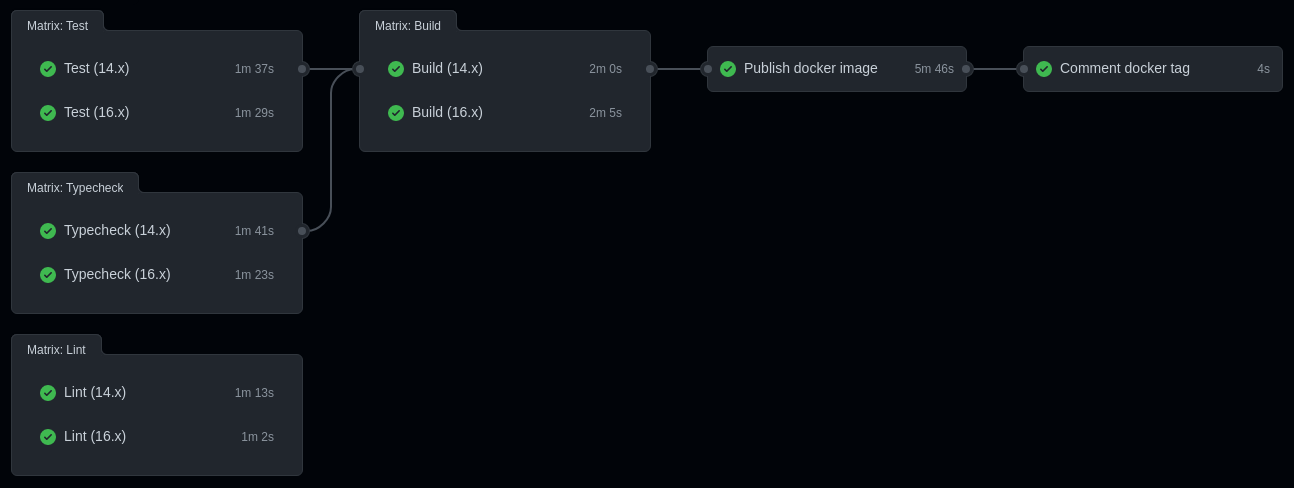
\includegraphics[width=0.6\textwidth]{images/github-actions-diagram.png}
    \caption{Propojení jednotlivých akcí v Github actions}

\end{figure}
Sem přijde schéma Github actions